% The listwise readout: one prompt -> one forward pass -> label probabilities -> new order.
% Shared by the technical report (Figure 1) and the repository README (rendered to PNG).
% Illustrative: the bar lengths are not measured values.
\documentclass[tikz, border=0pt]{standalone}
\usepackage[T1]{fontenc}
\usepackage[type1, sfdefault]{noto-sans}
\usepackage[type1, scale=0.92]{noto-mono}
\usetikzlibrary{arrows.meta, positioning, calc, shadows.blur}
% Colours, the gradient and the target icon shared by the report style and the standalone figures.
% \input by techreport.sty users and by the standalone figures. Needs xcolor and tikz.
\definecolor{jevink}{HTML}{1F1F1F}
\definecolor{jevmuted}{HTML}{444746}
\definecolor{jevsubtle}{HTML}{5E6368}
\definecolor{jevline}{HTML}{DDE3EA}
\definecolor{jevline2}{HTML}{E3E8EF}
\definecolor{jevfill}{HTML}{F0F4F9}
\definecolor{jevground}{HTML}{F8FAFD}
\definecolor{jevlink}{HTML}{0B57D0}
\definecolor{jevblue}{HTML}{4285F4}
\definecolor{jevpurple}{HTML}{9B72CB}
\definecolor{jevrose}{HTML}{D96570}
\definecolor{jevred}{HTML}{EA4335}
\definecolor{jevyellow}{HTML}{FBBC04}
\definecolor{jevgreen}{HTML}{34A853}
\pgfdeclarehorizontalshading{jevgrad}{100bp}{color(0bp)=(jevblue); color(25bp)=(jevblue); color(52bp)=(jevpurple);
  color(75bp)=(jevrose); color(100bp)=(jevrose)}
% the target icon, at height #1
\newcommand{\jevtarget}[1]{%
  \tikz[baseline=-0.5ex]{\draw[jevrose, line width=#1*0.12] (0,0) circle[radius=#1*0.38]; \fill[jevrose] (0,0) circle[radius=#1*0.18];}}

\newcommand{\semib}{\fontseries{sb}\selectfont}
\begin{document}
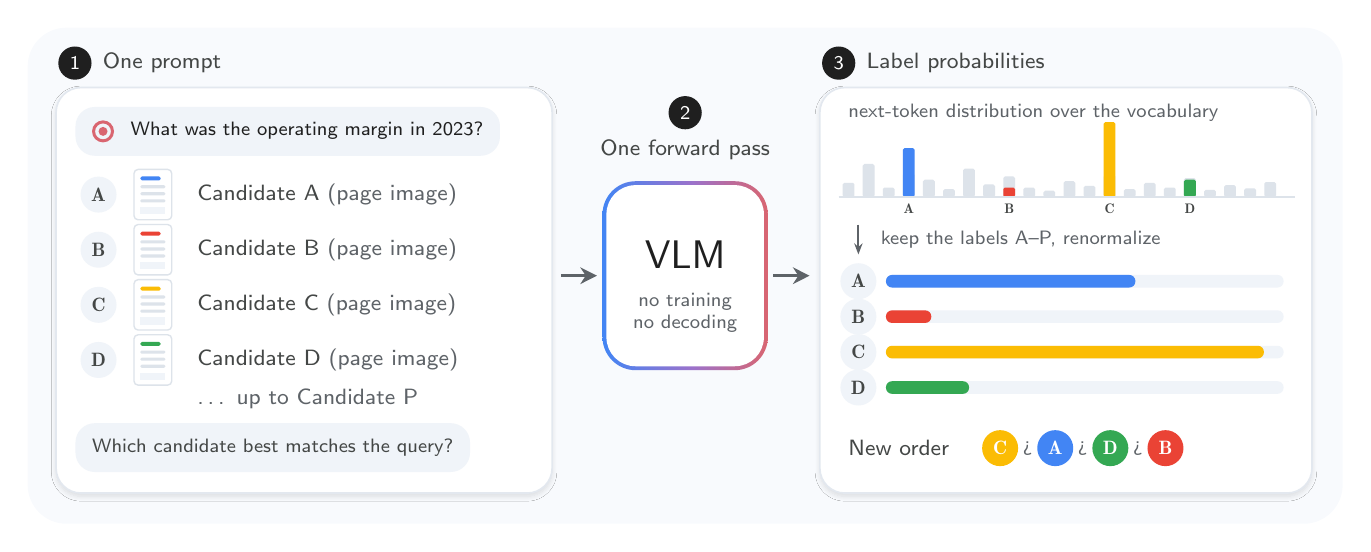
\begin{tikzpicture}[
    font=\sffamily\small, text=jevink,
    card/.style={fill=white, draw=jevline2, line width=0.6pt, rounded corners=9pt,
                 blur shadow={shadow blur steps=8, shadow xshift=0pt, shadow yshift=-1.2pt, shadow opacity=12}},
    chip/.style={fill=jevfill, rounded corners=7pt, inner ysep=0pt},
    lab/.style={circle, minimum size=13pt, inner sep=0pt, font=\notomono\scriptsize\semib},
    steptitle/.style={font=\sffamily\footnotesize\semib, text=jevmuted},
    num/.style={circle, fill=jevink, text=white, minimum size=12pt, inner sep=0pt, font=\sffamily\scriptsize\semib},
    flow/.style={-{Stealth[length=6pt, width=6pt]}, line width=1.1pt, draw=jevsubtle},
  ]
  % ---------------------------------------------------------------- canvas
  \fill[jevground, rounded corners=14pt] (-0.35,0.2) rectangle (16.35,6.5);

  % ---------------------------------------------------------------- 1. one prompt
  \node[num] at (0.25,6.05) {1};
  \node[steptitle, anchor=west] at (0.48,6.05) {One prompt};
  \node[card, minimum width=6.3cm, minimum height=5.15cm, anchor=north west] (p) at (0,5.75) {};
  % query chip
  \node[chip, anchor=north west, minimum height=0.62cm, inner xsep=6pt, font=\sffamily\fontsize{7.4}{9}\selectfont] (q) at (0.25,5.5)
       {\jevtarget{9pt}\hspace{6pt}What was the operating margin in 2023?};
  % candidates: label, page thumbnail, name
  \foreach \L/\c/\y in {A/jevblue/4.38, B/jevred/3.68, C/jevyellow/2.98, D/jevgreen/2.28} {
    \node[lab, fill=jevfill, text=jevmuted] at (0.55,\y) {\L};
    \begin{scope}[shift={(1.0,\y-0.32)}]
      \draw[jevline, fill=white, line width=0.5pt, rounded corners=1.5pt] (0,0) rectangle (0.48,0.64);
      \fill[\c, rounded corners=0.6pt] (0.08,0.5) rectangle (0.34,0.55);
      \foreach \yy in {0.40,0.31,0.22} \fill[jevline, rounded corners=0.5pt] (0.08,\yy) rectangle (0.40,\yy+0.04);
      \fill[jevfill] (0.08,0.07) rectangle (0.40,0.16);
    \end{scope}
    \node[anchor=west, font=\sffamily\footnotesize, text=jevmuted] at (1.68,\y) {Candidate \L\ \textcolor{jevsubtle}{(page image)}};
  }
  \node[anchor=west, font=\sffamily\footnotesize, text=jevsubtle] at (1.68,1.78) {\dots\ up to Candidate P};
  % question line
  \node[chip, anchor=south west, minimum height=0.62cm, inner xsep=6pt, font=\sffamily\fontsize{7.4}{9}\selectfont, text=jevmuted]
       (qq) at (0.25,0.85) {Which candidate best matches the query?};
  % report the chips' right edges: both must stay inside the card (right edge 6.3 cm, inner padding 0.25 cm)
  \path (q.east); \pgfgetlastxy{\qx}{\qy}\typeout{CHIPEAST q=\qx}
  \path (qq.east); \pgfgetlastxy{\qx}{\qy}\typeout{CHIPEAST qq=\qx}

  % ---------------------------------------------------------------- 2. one forward pass
  \node[num] at (8.0,5.42) {2};
  \node[steptitle, anchor=center] at (8.0,4.95) {One forward pass};
  \shade[shading=jevgrad, rounded corners=12pt] (6.95,2.15) rectangle (9.05,4.55);
  \fill[white, rounded corners=10.5pt] (7.0,2.2) rectangle (9.0,4.5);
  \node[font=\sffamily\Large\semib] at (8.0,3.62) {VLM};
  \node[font=\sffamily\scriptsize, text=jevsubtle, align=center] at (8.0,2.88) {no training\\no decoding};
  \draw[flow] (6.42,3.35) -- (6.88,3.35);
  \draw[flow] (9.12,3.35) -- (9.58,3.35);

  % ---------------------------------------------------------------- 3. probabilities of the labels
  \node[num] at (9.95,6.05) {3};
  \node[steptitle, anchor=west] at (10.18,6.05) {Label probabilities};
  \node[card, minimum width=6.25cm, minimum height=5.15cm, anchor=north west] at (9.7,5.75) {};
  % next-token distribution over the vocabulary, label tokens in colour
  \node[anchor=west, font=\sffamily\scriptsize, text=jevsubtle] at (9.95,5.42) {next-token distribution over the vocabulary};
  \foreach \i/\h in {0/0.18,1/0.42,2/0.12,3/0.30,4/0.22,5/0.10,6/0.36,7/0.16,8/0.26,9/0.12,10/0.08,
                     11/0.20,12/0.14,13/0.28,14/0.10,15/0.18,16/0.12,17/0.24,18/0.09,19/0.15,20/0.11,21/0.19} {
    \fill[jevline, rounded corners=0.6pt] (10.0+\i*0.255,4.35) rectangle ++(0.15,\h);
  }
  \foreach \i/\h/\c/\L in {3/0.62/jevblue/A, 8/0.12/jevred/B, 13/0.95/jevyellow/C, 17/0.22/jevgreen/D} {
    \fill[\c, rounded corners=0.6pt] (10.0+\i*0.255,4.35) rectangle ++(0.15,\h);
    \node[font=\notomono\tiny\semib, text=jevmuted] at (10.075+\i*0.255,4.2) {\L};
  }
  \draw[jevline] (9.95,4.35) -- (15.75,4.35);
  \draw[-{Stealth[length=4pt]}, jevsubtle, line width=0.7pt] (10.2,4.0) -- (10.2,3.62);
  \node[anchor=west, font=\sffamily\scriptsize, text=jevsubtle] at (10.36,3.81) {keep the labels A--P, renormalize};
  % probabilities of the labels, one bar per candidate
  \foreach \L/\c/\w/\y in {A/jevblue/0.33/3.28, B/jevred/0.06/2.83, C/jevyellow/0.50/2.38, D/jevgreen/0.11/1.93} {
    \node[lab, fill=jevfill, text=jevmuted] at (10.2,\y) {\L};
    \fill[jevfill, rounded corners=2.2pt] (10.55,\y-0.08) rectangle (15.6,\y+0.08);
    \fill[\c, rounded corners=2.2pt] (10.55,\y-0.08) rectangle (10.55+\w*9.6,\y+0.08);
  }
    % the new order
  \node[anchor=west, font=\sffamily\footnotesize\semib, text=jevmuted] at (9.95,1.16) {New order};
  \foreach \L/\c/\x in {C/jevyellow/12.0, A/jevblue/12.7, D/jevgreen/13.4, B/jevred/14.1} {
    \node[lab, fill=\c, text=white] at (\x,1.16) {\L};
  }
  \foreach \x in {12.35,13.05,13.75} \node[font=\sffamily\scriptsize, text=jevsubtle] at (\x,1.16) {>};
\end{tikzpicture}
\end{document}
